\documentclass{article}
\usepackage[utf8]{inputenc}
\documentclass[12pt]{article}
%\usepackage[left=3cm, right=2.5cm, top=2.5cm, bottom=2.5cm]{geometry}e}
\usepackage[utf8]{inputenc}
\usepackage[spanish,english]{babel}
\usepackage{apacite}
\usepackage[round]{natbib}
\usepackage{hyperref}
\usepackage{float}
\usepackage{svg}
\usepackage[margin = 1in, top=2cm]{geometry}% Margins
\setlength{\parindent}{2em}
\setlength{\parskip}{0.2em}
\usepackage{setspace} % Setting the spacing between lines
\usepackage{amsthm, amsmath, amsfonts, mathtools, amssymb, bm} % Math packages 
\usepackage{svg}
\usepackage{graphicx}
\usepackage{pgfplots}
\usepackage{epstopdf}
%\usepackage{subfig} % Manipulation and reference of small or sub figures and tables
\usepackage{hyperref} % To create hyperlinks within the document
\spacing{1.15}
\usepackage{appendix}
\usepackage{xcolor}
\usepackage{cancel}
\usepackage{enumerate}
\usepackage{subcaption}
\usepackage[shortlabels]{enumitem}


\usepackage[round]{natbib}
%\bibliographystyle{plainnat}
\bibliographystyle{apacite}


\newtheorem{defin}{Definition.}
\newtheorem{teo}{Theorem. }
\newtheorem{lema}{Lemma. }
\newtheorem{coro}{Corolary. }
\newtheorem{prop}{Proposition. }
\theoremstyle{definition}
\newtheorem{examp}{Example. }
\newtheorem{problem}{Problem}
% \numberwithin{problem}{subsection} 

\newcommand{\card}{\operatorname{card}}
\newcommand{\qiq}{\qquad \implies \qquad}
\newcommand{\qiffq}{\qquad \iff \qquad}
\newcommand{\qaq}{\qquad \textbf{and} \qquad}
\newcommand{\qoq}{\qquad \textbf{or} \qquad}
\newcommand{\settf}{\text{ \emph{:} }}
\newcommand{\chbox}{\makebox[0pt][l]{$\square$}\raisebox{.15ex}{\hspace{.9em}}}
\newcommand{\cchbox}{\makebox[0pt][l]{$\square$}\raisebox{.15ex}{\hspace{0.1em}$\checkmark$}}

\title{Problem Set 3 711 Part 2}
\author{Mitchell Valdés-Bobes}
\date{November 14, 2020}

\begin{document}

\maketitle
\subsection*{Problem 1.}

\subsubsection*{Answer}
\newline
\textbf{(a)}

This means that the marginal valuation of weapons is greater that the fixed price per weapon. This guarantees a positive quantity of weapons is possible as an equilibrium.

\textbf{(b)}\newline This is game is super modular if:
\begin{itemize}
    \item $W_{i}$ is a compact subset of $\mathbb{R}$.
    \item $u_{i}$ is upper semi-continuous in $w_{i}, w_j$
    \item $u_{i}$ has increasing differences in $w_{i}, w_j$
\end{itemize}

The utility function is continuous in both arguments therefore it is upper-semi-continuous. The mixed second derivative of the utility function is:
$$\frac{\partial u}{\partial w_i \partial w_j} = 2 \beta -\frac{\alpha }{2} \geq 0 \qiffq \beta \geq \frac{\alpha}{4}$$

Then, the game if supermodular if $W_i$ is a compact set and $\beta \geq \frac{\alpha}{4}$.

\textbf{(c)}
Optimality conditions taking the other's gang strategy as given, gives:
$$\frac{\partial u}{\partial w_i}(w_i, w_j) = 0 \qiffq \operatorname{BR}_i(w_j) = \frac{2 \gamma -2 \rho -\alpha w_j+4 \beta  w_j}{2 (\alpha +2 \beta )}
$$

Note that any equilibrium in pure strategies is a solution of the following system of equations:

$$\left\{ \begin{array}{cc}
    w_i = \operatorname{BR}_i(w_j)   \\
    w_j = \operatorname{BR}_j(w_i) 
\end{array}$$

this give us the solution:

$$w_i = w_j = w^* = \frac{2(\gamma - \rho)}{3\alpha}$$

Thus we can conclude that the only equilibrium in pure strategies is the symmetric equilibrium, previously stated.

\textbf{(d)}
The effects of the parameters in the quantity of weapons in the symmetric equilibrium are:
\begin{itemize}
    \item $\beta$: No effect, since the equilibrium is symmetric the parameter that measures how much do each gang dislike having more weapons than the other, does not affect the quantity.
    \item $\gamma$: The equilibrium quantity is increasing in $\gamma$, since this is the parameter that captures the intrinsic valuation of weapons.
    \item $\alpha$, $\rho$: The equilibrium quantity is decreasing in both parameters, since weapons will be more costly when  $\alpha$ and $\rho$ are larger
\end{itemize}

\textbf{(e)}
The strategy of choosing $0$ weapons is no rationalizable since it is not a best response to any allowable conjecture, to see this re-write the best response as:
$$\operatorname{BR}_i(w_j) =  \frac{2(\gamma - \rho)+w_j(4\beta - \alpha)}{2 (\alpha +2 \beta )}$$
Then is clear to see that under the assumptions of the problem, namely:
$$w_i \geq 0 \qquad  \gamma > \rho \qquad \beta \geq \frac{\alpha}{4}$$
Best responses are always strictly positive. Since choosing $0$ weapons is not a rationalizable strategy, then there is no Nash equilibrium that involves that strategy. 

\textbf{(f)} By \cite{milgrom1990rationalizability} \textbf{Theorem 5} this game is dominance solvable therefore the only equilibrium is in pure strategies.

\textbf{(g)}
If both gangs have $w^*$ weapons, suppose that only gang 1 can respond to the goblin invasion (by moving to a new level $w^*
+\varepsilon$), we can re-write the problem as:

$$\max_{\varepsilon} \quad (w^*+\varepsilon)\left[\tilde{\gamma}-\rho-\alpha\left(w^*+\frac{\varepsilon}{2}\right)\right]-\beta \varepsilon^2 \qiq \varepsilon = \frac{-2 \tilde{\gamma} +2 \rho +\alpha  w^*}{2 (\alpha -2 \beta )}$$

Where $\tilde{\gamma} > \gamma $ is the new intrinsic valuation of weapons due to the invasion of goblins. Plug in the value of $w^*$ and we get the optimal increase in weapons for gang one:

$$\varepsilon = \frac{\tilde{\gamma} -\gamma}{\alpha +2 \beta }$$

To find the increase in weapons when both gangs are able to respond we will just compare the symmetric  equilibrium before and after the invasion. Call this increase $\hat{\varepsilon}$:
$$\varepsilon = \frac{2(\tilde{\gamma} - \rho)}{3\alpha}- \frac{2(\gamma - \rho)}{3\alpha} = \frac{2(\tilde{\gamma} - \gamma)}{3\alpha}$$

Since $4\beta \geq \alpha$ then $\varepsilon > \hat{\varepsilon}$, meaning that when only one gang is able to adjust the increase in weapons will be higher.

\section{Question 2}
\subsubsection*{Answer}

To find symmetric pure strategy Nash equilibrium we start by finding the best response to any average weapons quantity:
$$\operatorname{BR}_i(\bar{w}) = \frac{\gamma - \rho + \bar{w}(2\beta - \alpha)}{2\beta}$$

Since we are looking for symmetric equilibria we can solve:

$$\operatorname{BR}_i(\bar{w}) = \bar{w} \qiq w_i = \frac{\gamma - \rho}{\alpha} $$

The equilibrium quantity is greater because since each gang has no market power (unlike \textbf{Problem  1}) then they all think that their choice won't drive up the price, therefore to have more weapons.

\section*{Question 3}
\begin{proof}[Answer:]
\textbf{(a)}Another way to write the utility is 
$u_i(x_i, \bar{x},\alpha)=(x-\alpha)(2 x_i - \alpha -\bar{x}) $
We can easily see that since $x_i \in [0,1]$ the best reply function is
\begin{equation}
BR_i(\bar{x}, \alpha) =\begin{cases} 
      0 & \text{if } \alpha < \bar{x}  \\
      \Delta\{0,1\} &  \text{if }\alpha = \bar{x} \\
      1 &  \text{if } \alpha < \bar{x}  
   \end{cases}
\end{equation}
Now we look for symmetric pure NE: all players $i$ play $x_i$ (which implies  $x_i= \bar{x}$ ), then we divide the search in three cases
\begin{enumerate}
    \item when $x_i = \bar{x} < \alpha$:
If $x_i>0$ there is a contradiction since one player has incentives to deviate to 0. Hence, the following is NE
$$x_i= 0$$ 
      \item when $x_i = \bar{x} = \alpha$: 
      Payoffs are always 0, so no player will move so it is NE: $$x_i  = \alpha$$
      
        \item when $x_i = \bar{x} < \alpha$:
        
        Using the same logic that 1., the NE is $$x_i = 1$$
        \end{enumerate}
\textbf{(b)} Let $Q(x)$ be a quantile function. The unique property that this cdf must have is
$$\mathbb{E}[x] = \alpha$$
Furthermore, every quantile function with this property is a NE.

Whenever $\mathbb{E}[x] < \alpha$ ($\bar{x}<\alpha$), any strategy $z$ in the support of $Q$, such that  $z<\alpha$, is worst than $x = 0$. Likewise, if $\bar{x}>\alpha$ we know that $x = 1$ has a higher payoff. If $$\mathbb{E}[x] = \alpha$$, every $z$ in the support of $Q$, yields a utility of 0, as well as any other strategy $x$, thus this strategy is optimal.

\textbf{(c)} In this case the largest and smallest  symmetric NE  that we have $x_i = 1$ and $x_i = 0$ are not and equilibrium in this case. Not only for 0, 1, but for any other $x_l$ and $x_s$, since there is always a smaller and largest strategy. 

$x_i = \alpha $ for all $i$ is still a symmetric pure NE.

The proof that we give in b) hold in this case so $Q$ with this properties is a NE.
\end{proof}
\section*{Question 4}

Player $i$'s best response to any selection of player $j$ is:
$$\operatorname{BR}_(q_j) = 1 + (1-q_j)^{1/3}$$
This means that there are 3 pure strategy equlibria, as shown in the following figure:

\begin{center}
    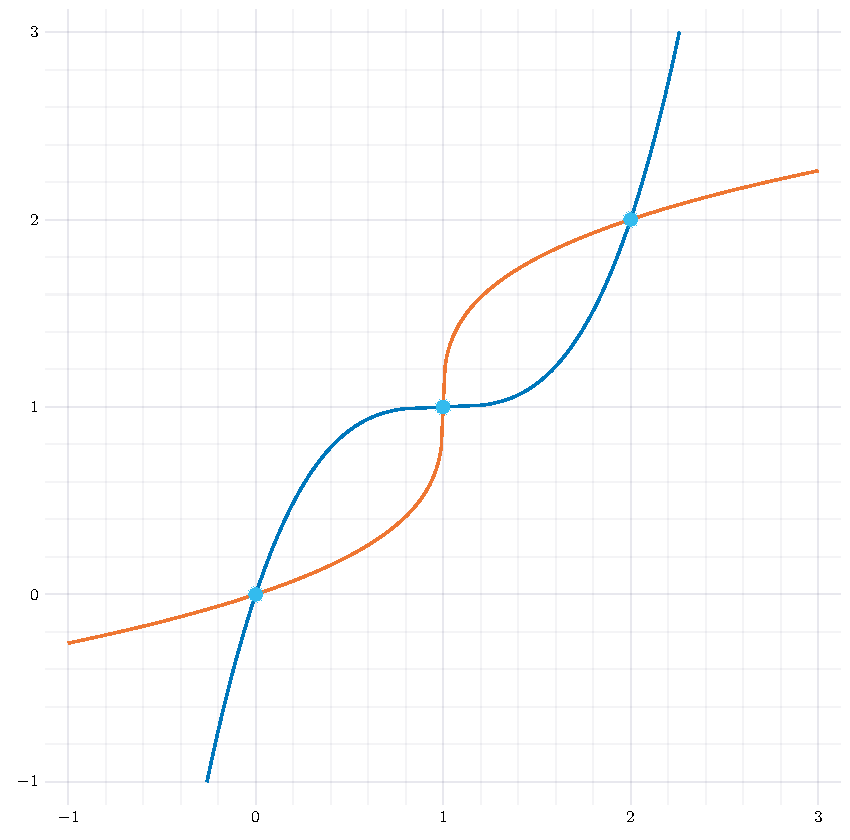
\includegraphics[scale=.4]{fig_ps2.pdf}   
\end{center}

Solving the FOC, it is was easy to see that the points that correspond to the symmetric equilibrium are those where both players choose $0$, $1$ and $2$.

Since the utility function is strictly concave in her own action then each player will be strictly better-off by choosing a pure strategy no matter what the other player does; this means that the symmetric Nash equilibria in pure strategies previously discussed are the only possible equilibria for this game.

\section*{Question 5}

\begin{proof}
One way in which we can model this game is
\begin{itemize}
    \item $N = \{1,2\}$
    \item Strategies are stochastic vectors, $\alpha \in [0,1]^3 : \sum_i \alpha_i = 1$ 
    \item The utility is 
    $$U_i(\alpha_i,\alpha_j) =
      u_i(\alpha_i,\alpha_j) $$
      where $$C(\alpha_i) = \begin{cases} 
      0 & \text{if }\alpha_i \in \{(1,0,0),(0,1,0),(0,0,1)\}  \\
      1 & \text{otherwise}
   \end{cases}
$$ 
\end{itemize}

We only need to check the NE of the original game. See that pure strategies NE are not possible in this competitive game. Mixed-strategy equilibrium where randomization occur in 2 actions does not exist, since this give us the same contradictions that in the original game. The unique NE in the original game comes from solving the indifference conditions: 

$$\alpha_S-\alpha_P =\alpha_R-\alpha_S =\alpha_P-\alpha_R $$  
$$\alpha_P+\alpha_R+\alpha_S = 1$$
This give us that both player choose to play
$$\alpha^*=\left(\frac{1}{3},\frac{1}{3},\frac{1}{3}\right)$$
And this is no worst than any other strategy in the original game.

In the current game, the utility of playing any strategy in $X= \{(1,0,0),(0,1,0),(0,0,1)\}$
$$U_i(x,\alpha^*) = 0 > -1 = U_i(\alpha^*,\alpha^*), x\in $
This is thus not a NE and therefore we have no NE in this game since we have exhausted all possibilities. See that randomizing here give us the same utility that a simple lottery.

\end{proof}



\end{document}
